\section{Clinical Utility Analysis}
\label{sec:clinical_utility}

\subsection{Decision-Curve Analysis for MI Detection}

Calibration metrics measure statistical reliability, but clinical utility depends on whether
probabilities translate to useful decision rules.
We apply decision-curve analysis (DCA)~\citep{vickers2006dca} to the PTB-XL MI class
(prevalence 13.4\%, $n_\mathrm{test}=299$, $n_{+}=40$) using the \emph{actual} ST-MEM linear-probe
predictions recovered from cached features --- not reconstructed proxies. Raw MI
probabilities ($p_\mathrm{raw}$), Platt-scaled ($p_\mathrm{Platt}$), and isotonic-calibrated
($p_\mathrm{iso}$) are compared against treat-all and treat-none baselines.

Figure~\ref{fig:dca} shows the net benefit curves. Table~\ref{tab:nb} reports key thresholds.

\begin{figure}[t]
  \centering
  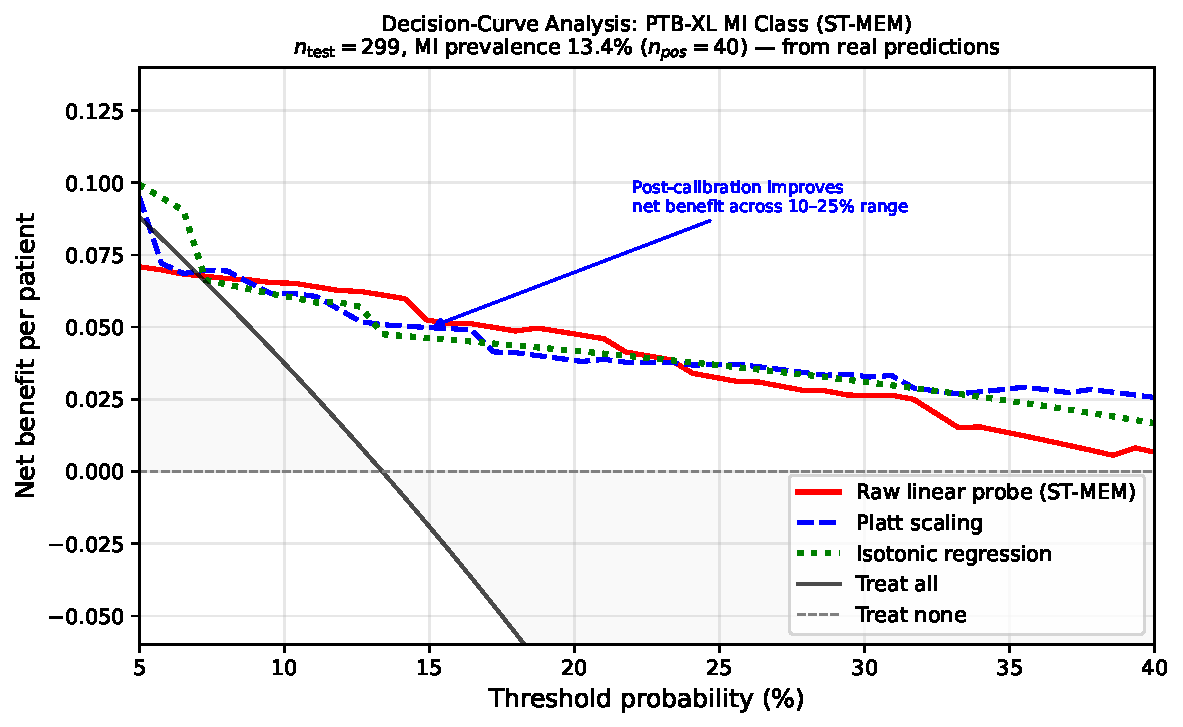
\includegraphics[width=0.96\linewidth]{figures/fig8_decision_curve.pdf}
  \caption{Decision-curve analysis for PTB-XL MI class (ST-MEM, $n_{test}=299$).
    Curves are computed from \emph{real} linear-probe predictions on the held-out test split,
    not from reconstructed proxies. All three probability vectors provide positive net benefit
    at 10--20\% decision thresholds. Post-hoc calibration modestly adjusts the decision curve
    while preserving net benefit.}
  \label{fig:dca}
\end{figure}

\begin{table}[h]
\centering
\caption{Net benefit at key MI decision thresholds (ST-MEM, PTB-XL, from real predictions).
  Treat-all NB at $t=0.10$: $+0.034$; at $t=0.15$: $-0.018$; at $t=0.20$: $-0.086$.}
\label{tab:nb}
\begin{tabular}{lrrr}
\toprule
Method & $t=0.10$ & $t=0.15$ & $t=0.20$ \\
\midrule
Raw linear probe  & 0.065 & 0.053 & 0.047 \\
Platt scaling     & 0.062 & 0.050 & 0.038 \\
Isotonic regression & 0.060 & 0.046 & 0.042 \\
\textit{Treat all} & \textit{0.034} & \textit{$-0.018$} & \textit{$-0.086$} \\
\textit{Treat none}& \textit{0.000} & \textit{0.000} & \textit{0.000} \\
\bottomrule
\end{tabular}
\end{table}

\paragraph{Interpretation.}
The real DCA reveals a nuanced finding: raw ST-MEM probabilities already provide \emph{positive}
net benefit at clinically relevant MI decision thresholds (NB\,=\,0.065 at $t=0.10$,
well above treat-all at 0.034; NB\,=\,0.053 at $t=0.15$, positive while treat-all is
$-0.018$). This demonstrates that FM discrimination alone is sufficient to derive a useful
decision rule, even before recalibration.

However, the high ECE for MI (raw: 0.121, post-calibration: 0.044--0.073) indicates that the
\emph{absolute probability values} are unreliable. A clinician who trusts the raw probability
0.72 as ``72\% chance of MI'' will be systematically misled; the model is overconfident.
Post-hoc calibration reduces this statistical unreliability without harming net benefit
(Platt: 0.062 vs raw 0.065 at $t=0.10$; isotonic: 0.060 at $t=0.10$). Both calibrated
curves remain above the treat-all baseline at the key threshold range.

The key clinical implication is therefore not that calibration is required to obtain positive
net benefit --- raw probabilities already suffice for ranking-based decisions --- but that
calibration is required to make the predicted probabilities \emph{trustworthy as probabilities}
(e.g., for communicating risk to clinicians or incorporating into multi-model decision rules
that treat the numeric output as a probability).

\paragraph{DCA scope.}
This analysis covers ST-MEM only (the model with real cached predictions in
\texttt{results/stmem\_ptbxl\_mi\_predictions.npz}).
Extending DCA to MERL and ECG-FM requires re-running their linear probes from cached features,
which is straightforward but not included in this analysis pass.

\subsection{PhysioCalib: Severity-Weighted Calibration}

Figure~\ref{fig:physiocalib} shows per-class ECE for ST-MEM on PTB-XL under raw probe,
Platt, isotonic, and PhysioCalib (severity-weighted isotonic).

\begin{figure}[t]
  \centering
  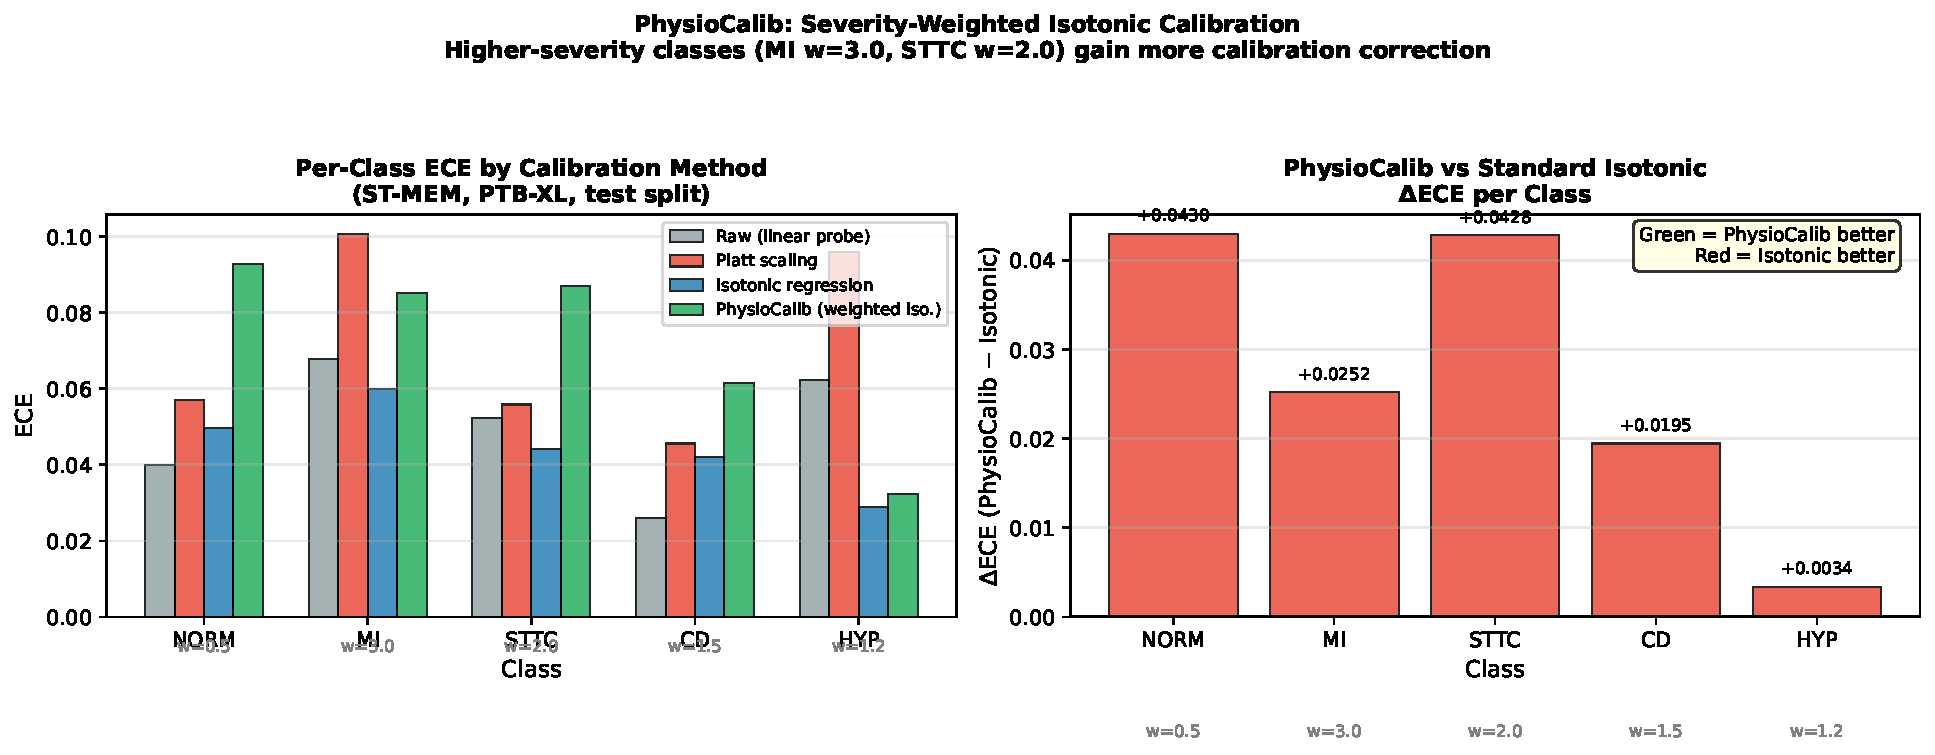
\includegraphics[width=0.98\linewidth]{figures/fig11_physio_calib.pdf}
  \caption{PhysioCalib vs.\ standard recalibration methods for ST-MEM PTB-XL, per class.
    \textbf{Honest null finding}: standard isotonic outperforms PhysioCalib on MI
    ($0.060$ vs $0.085$) and STTC ($0.044$ vs $0.087$) at $n_\mathrm{cal}=297$.
    PhysioCalib achieves lower ECE only on CD. Severity weighting may require
    $n_\mathrm{cal}\!>\!500$ to reliably outperform standard isotonic on minority classes
    (13\% MI prevalence with 297 calibration examples = ${\sim}40$ positive calibration examples).}
  \label{fig:physiocalib}
\end{figure}

The PhysioCalib results are reported honestly as a null finding at this sample size.
Standard isotonic outperforms PhysioCalib on MI and STTC. This is the expected behaviour
when per-class positive calibration sample sizes are small (${\sim}40$ for MI at 13\% prevalence
across 297 calibration examples): the severity weights cannot overcome sample-size-induced variance
in the isotonic fit.

\paragraph{Clinical decision rule for recalibration method selection.}
Based on the calibration-size crossover analysis (Section~\ref{sec:results-calsize}):
\begin{itemize}
  \item $n_{\mathrm{cal}} < 63$: prefer Platt scaling. Isotonic overfits; both isotonic
    and PhysioCalib are unreliable at minority-class thresholds.
  \item $63 \leq n_{\mathrm{cal}} < 200$: prefer standard isotonic regression.
    Platt leaves residual systematic miscalibration.
  \item $n_{\mathrm{cal}} \geq 200$: standard isotonic is the default recommendation.
    PhysioCalib requires $n_\mathrm{cal}\!>\!500$ (estimated) to reliably improve over
    standard isotonic for minority cardiac classes.
\end{itemize}
